\documentclass{report}
\usepackage{amsmath}
\usepackage{amssymb}
\usepackage{multirow}
\usepackage[margin=0.75in]{geometry}
\usepackage{fancyhdr}
\usepackage{etoolbox}
\usepackage{amsthm}
\usepackage{calc}
\usepackage{tikz,pgfplots}
\usepackage{graphicx}
\usepackage{rotating}
\usepackage{stackengine}
\usepackage{tcolorbox}
\usetikzlibrary{arrows}
\usepackage{array,booktabs,arydshln,xcolor}
\usepgfplotslibrary{fillbetween}
\pgfplotsset{compat=1.16,width=10cm}





%% New colors

\definecolor{darkgreen}{rgb}{0.0, 0.4, 0.2}

%%Section and chapter references macros
%%%%%%%%%%%%%%%%%%%

\makeatletter
\newcommand*{\currentname}{\@currentlabelname}
\makeatother

\newcommand\getcurrentref[1]{%
 \ifnumequal{\value{#1}}{0}
  {??}
  {\the\value{#1}}%
}    

\newcommand{\longdivision}[2]{
    \settowidth{\dividendlength}{#1}
    \settowidth{\divisorlength}{#2}
    \settoheight{\dividendheight}{#1}
    \settoheight{\maxheight}{#1#2}
    \settoheight{\divisorheight}{#2}

    \begin{tikzpicture} [baseline=.5pt]
        \node at (-.5*\divisorlength-1pt,.5*\divisorheight) {#2};
        \node at (.5*\dividendlength+5pt,.5*\dividendheight) {#1};
        \draw [thick]  (0pt,-.22*\dividendheight) arc (-70:60:\maxheight*.41 and \maxheight*.82) -- ++(\dividendlength+7pt,0pt);
    \end{tikzpicture}
}

\newlength{\dividendlength}
\newlength{\divisorlength}
\newlength{\dividendheight}
\newlength{\divisorheight}
\newlength{\maxheight}

%%%%%%%Commands%%%%%%%%%%%%%%%%%%%%%
\theoremstyle{definition}
\newtheorem{example}{\bf Example}
\newtheorem{youtry}{\bf You Try It!}
\newtheorem{definition}{\bf Definition}[section]
\newtheorem{theorem}{\bf Theorem}[section]




%%%%%%%%%%%%%Header%%%%%%%%%%%%%%%%%%%
\pagestyle{fancy}
\fancyhf{}
\renewcommand{\headrulewidth}{0pt}
\lhead{}
\rhead{Algebra 2: Section  \getcurrentref{chapter}.\getcurrentref{section}}
\cfoot{ }
\rfoot{Page \thepage}
%%%%%%%%%%%%%%%%%%%%%%%%%%%%%%%%%%%%%%

%% Set start page here 
\setcounter{page}{1}



%%% Set Chapter counter here
\setcounter{chapter}{7}
\setcounter{section}{0}


%%%%%%%%%%%%%%% New Section Template %%%%%%%%%%%%%%%%
%%%%%%%%%%%%%%%%%%%%%%%%%%%%%%%%
%%%%%%%%%%%%%%%%%%%%%%%%%%%%%%%%
%%%%%%%   Section _._   %%%%%%%%
%%%%%%%%%%%%%%%%%%%%%%%%%%%%%%%%
%%%%%%%%%%%%%%%%%%%%%%%%%%%%%%%%
% \section{    NAME HERE   }
% \setcounter{example}{0}
% \setcounter{definition}{0}
% %%%%%%%%%%%%%%%%%%%%%%%%%%%%%%%%
% %%%%%%%%%%%%%%%%%%%%%%%%%%%%%%%%
% \begin{definition}
%     Definition
% \end{definition}
% \begin{example}
%     Example
% \end{example}
%
%\vspace{-0.5cm}
%\hspace{-0.5cm}
%%
%% LeftOfPage%%%%%
%\begin{minipage}{0.45\linewidth}
% \begin{itemize}
%     \item[(a)]
% \end{itemize}
%%
%\vspace{2.75cm}
%%
% \begin{itemize}
%     \item[(c)]
% \end{itemize}
%%
%\vspace{2.75cm}
%%
%\end{minipage}
%\hspace{1.5cm}
%%RightOfPage%%%%%
%\begin{minipage}{0.45\linewidth}
% \begin{itemize}
%     \item[(b)]
% \end{itemize}
%%
%\vspace{2.75cm}
%%
% \begin{itemize}
%     \item[(d)]
% \end{itemize}
%%
%\vspace{2.75cm}
%%
%\end{minipage}
%%%%%%%%%%%%%%%%%%%%%%
%
%%%%%%%%%%%%%%%%% Example 2
%\begin{example}
%     Use \textbf{elimination} to solve each system of equations.
%\end{example}
%%
%\vspace{-0.5cm}
%\hspace{-0.5cm}
%%
%% LeftOfPage%%%%%
%\begin{minipage}{0.45\linewidth}
% \begin{itemize}
%     \item[(a)]
% \end{itemize}
%%
%\vspace{2.75cm}
%%
% \begin{itemize}
%     \item[(c)]
% \end{itemize}
%%
%\vspace{2.75cm}
%%
%\end{minipage}
%\hspace{1.5cm}
%%RightOfPage%%%%%
%\begin{minipage}{0.45\linewidth}
% \begin{itemize}
%     \item[(b)]
% \end{itemize}
%%
%\vspace{2.75cm}
%%
% \begin{itemize}
%     \item[(d)]
% \end{itemize}
%%
%\vspace{2.75cm}
%%
%\end{minipage}
%%%%%%%%%%%%%%%%%%%%%
%\vfill
% \noindent\fbox{\large\textbf{_._ Homework}: page \small }
%%%%%%%%%%%%%%%%%%%%%%%%%%%%%%%%%%%%%%
%%%%%%%%%%%%%%%%%%%%%%%%%%%%%%%%%%%%%%
% \newpage
%%%%%%%%%%%%%%%%%%%%%%%%%%%%%%%%%%%%%%
%%%%%%%%%%%%%%%%%%%%%%%%%%%%%%%%%%%%%%



% number line example%%%%
%\begin{tikzpicture}
        %\draw[latex-latex] (-3.5,0) -- (3.5,0) ; %edit here for the axis
        %\foreach \x in  {-3,-2,-1,0,1,2,3} % edit here for the vertical lines
        %\draw[shift={(\x,0)},color=black] (0pt,3pt) -- (0pt,-3pt);
        %\foreach \x in {-3,-2,-1,0,1,2,3} % edit here for the numbers
        %\draw[shift={(\x,0)},color=black] (0pt,0pt) -- (0pt,-3pt) node[below] 
        %{$\x$};
        %\draw[*-o] (0.92,0) -- (2.08,0);
        %\draw[very thick] (0.92,0) -- (1.92,0);
%\end{tikzpicture}



\setcounter{section}{-1}
\begin{document}

\noindent\LARGE\textbf{Chapter 7 Exponential Logarithmic Functions}\normalsize

%%%%%%%%%%%%%%%%%%%%%%%%%%%%%%%
%%%%%%%%%%%%%%%%%%%%%%%%%%%%%%%
%%%%%%   Section 7.0   %%%%%%%%
%%%%%%%%%%%%%%%%%%%%%%%%%%%%%%%
%%%%%%%%%%%%%%%%%%%%%%%%%%%%%%%
\rhead{Algebra 2: Section  \getcurrentref{chapter}.0}
 \section{Pre-assessment }
 \setcounter{section}{0}
 \setcounter{example}{0}
 \setcounter{definition}{0}
 %%%%%%%%%%%%%%%%%%%%%%%%%%%%%%%%
 %%%%%%%%%%%%%%%%%%%%%%%%%%%%%%%%
 \vspace{0.5cm}
 
\textbf{Match each of the vocabulary terms on the left with the appropriate letter and definition on the right.}\\

\begin{enumerate}
	\begin{minipage}[t]{0.25\linewidth}
	
			\item exponent.
				\vspace{0.7cm}
			\item function.
				\vspace{0.7cm}
			\item relation.
				\vspace{0.7cm}
			\item variable.
				\vspace{0.7cm}
	
	\end{minipage}
	\begin{minipage}[t]{0.65\linewidth}
		\begin{itemize}
			\item[A.] a symbol used to represent one or more numbers.
				\vspace{0.25cm}
			\item[B.] the set of counting numbers and their opposites
				\vspace{0.25cm}
			\item[C.] a relation with at most one $y$-value for each $x$-value.
				\vspace{0.25cm}
			\item[D.] the number of times the base of a power is used as a factor.
				\vspace{0.25cm}
			\item[E.] a set of ordered pairs.
				\vspace{0.25cm}
		\end{itemize}
	\end{minipage}
\end{enumerate}
\noindent \textbf{Simplify each expression.}\\

\begin{enumerate}
\setcounter{enumi}{4}
	\begin{minipage}[t]{0.225\linewidth}
	\item $x^2(x^3)(x)$
	\end{minipage}
	\begin{minipage}[t]{0.225\linewidth}
	\item $3y^{-1}(5x^2y^2)$
	\end{minipage}
	\begin{minipage}[t]{0.225\linewidth}
	\item $\displaystyle \frac{a^{-2}b^3}{a^4b^{-1}}$.
	\end{minipage}
	\begin{minipage}[t]{0.225\linewidth}
	\item $(3x)^2(4x^3)$
	\end{minipage}
\end{enumerate}

\vspace{2cm}

\noindent \textbf{Use the simple interest formula, $I=Prt$, where $I$ is the interest, $P$ is the initial amount (principal), and $r$ is the interest rate..}\\

\begin{enumerate}
\setcounter{enumi}{8}
		\item Find the simple interest on an investment of $\$3000$ at $3\%$ for 2 years..
			\vfill
		\item A savings account of $\$2000$ earned $\$90$ simple interest in 3 years. Find the interest rate.
			\vfill
\end{enumerate}

\noindent \textbf{Solve each equation for x.}\\

\begin{enumerate}
\setcounter{enumi}{10}
	\begin{minipage}[t]{0.45\linewidth}
	\item $\displaystyle \frac{x}{2}=3y-4$
	\end{minipage}
	\begin{minipage}[t]{0.45\linewidth}
	\item $\displaystyle  y=\frac{3}{4}x-\frac{1}{2}$
	\end{minipage}
\end{enumerate}
\vfill
\begin{flushright}
\rotatebox{180}{\color{red}10. $1.5\%$ 11. $6y-8$ 12. $(4y+2)/3$\color{black}   }\\
\vspace{0.5cm}
\rotatebox{180}{\color{red}1. D \, 2. C\, 3. E\, 4. A\,  5. $x^6$\, 6. $15x^2y$\, 7. $b^4/a^6$\, 8. $36x^5$\,  9. $\$180$ \color{black}}
\end{flushright}
	
%%%%%%%%%%%%%%%%%%%%%%%%%%%%%%%%%%%%%
%%%%%%%%%%%%%%%%%%%%%%%%%%%%%%%%%%%%%
 \newpage
%%%%%%%%%%%%%%%%%%%%%%%%%%%%%%%%%%%%%
%%%%%%%%%%%%%%%%%%%%%%%%%%%%%%%%%%%%%

%%%%%%%%%%%%%%%%%%%%%%%%%%%%%%%
%%%%%%%%%%%%%%%%%%%%%%%%%%%%%%%
%%%%%%   Section 7.1   %%%%%%%%
%%%%%%%%%%%%%%%%%%%%%%%%%%%%%%%
%%%%%%%%%%%%%%%%%%%%%%%%%%%%%%%
\rhead{Algebra 2: Section  \getcurrentref{chapter}.\getcurrentref{section}}
\setcounter{section}{0}
 \section{ Exponential Functions, growth and Decay }
 \indent\hfill\small\noindent \textbf{Objective}: Write and evaluate exponential expressions to model growth and decay situations. \normalsize\\
 \vspace{-0.5cm}
 \setcounter{example}{0}
 \setcounter{definition}{0}
 %%%%%%%%%%%%%%%%%%%%%%%%%%%%%%%%
 %%%%%%%%%%%%%%%%%%%%%%%%%%%%%%%%

\vspace{1cm}

\noindent Moore's law, a rule used in the computer industry, states that the number of transistors per integrated circuit (the processing power) doubles every year. Beginning in the early days of integrated circuits, the growth in capacity may be approximated by this table.

\begin{center}
	\begin{tabular}[t]{|l|c|c|c|c|c|c|c|}
		\hline
		\multicolumn{8}{|c|}{}\\
		\multicolumn{8}{|c|}{\textbf{Transistors per Integrated Chip}}\\
		\hline
		&&&&&&&\\
		Year&1965&1966&1967&1968&1969&1970&1971\\
		\hline
		&&&&&&&\\
		Transistors&60&120&240&480&960&1920&3840\\
		\hline
		\multicolumn{8}{c}{}\\
		\multicolumn{1}{c}{}&\multicolumn{7}{c}{$\color{red}\qquad\times 2 \quad\,\, \times 2 \quad\,\,\, \times 2 \quad\,\, \times 2 \quad\,\, \times 2 \quad\,\,\, \times 2 \quad\,\,$\color{black}}\\
	\end{tabular}
\end{center}


\begin{definition}
Functions with a variable exponent are known as \textbf{exponential functions}. The parent exponential function is $f(x)=b^x$, where the \textbf{base} $b$ is a constant and the exponent $x$ is the independent variable.
\end{definition}

\Large
\[f(x)=\color{blue}b\color{red}^{x}\color{black}\text{, where \color{blue} $b>0$ \color{black},\color{blue} $b\neq 1$.}\]
\normalsize


\begin{minipage}[t]{0.45\linewidth}
\vspace{-6.25cm}
	\begin{tabular}[t]{|c|c|c|c|c|c|c|}
	\hline
	&&&&&&\\
	$\mathbf{x}$&-2&-1&0&1&2&3\\
	&&&&&&\\
	\hline
	&&&&&&\\
	$\mathbf{f(x)=2^x}$ & \qquad\qquad &  \qquad\qquad & \qquad\qquad & \qquad\qquad & \qquad\qquad & \qquad\qquad \\
	&&&&&&\\
	\hline
	\end{tabular}
\end{minipage}
\hfill
\begin{minipage}[t]{0.45\linewidth}
	 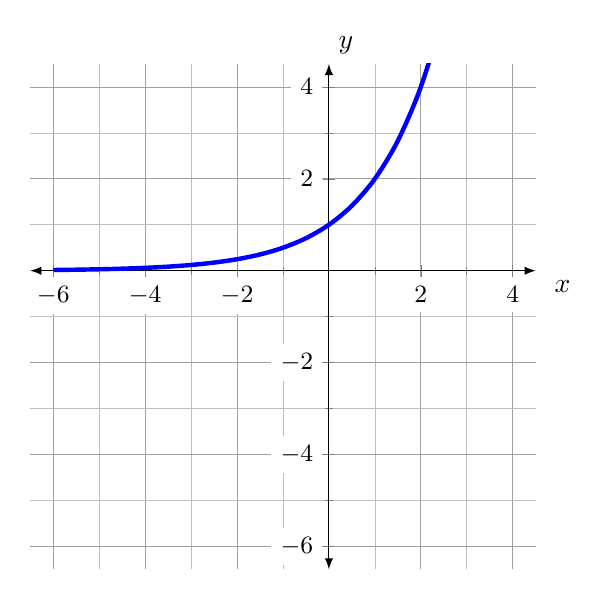
\begin{tikzpicture}[>=latex,scale=1]
			\begin{axis}[
					    width =8cm,
				               height=8cm,
					    xmin=-6,xmax=4,
					    ymin=-6,ymax=4,
					    grid=both,
					    grid style={line width=.2pt, draw=gray!50},
					    major grid style={line width=.3pt,draw=gray!75},
					    axis lines=middle,
					    minor tick num=1,
					    enlargelimits={abs=0.5},
					    axis line style={latex-latex},
					    ticklabel style={font=\small,fill=white},
					    xlabel={\,\,$x$},
					    ylabel={$y$},
					    xlabel style={below right},
					    ylabel style={above right},
					]
					\addplot[domain=-6:6, blue, ultra thick, smooth] {2^x};
			\end{axis}	
	\end{tikzpicture}
\end{minipage}

\vfill

\begin{definition}
An \textbf{asymptote} is a line that a graphed function approaches as the value of $x$ gets very large or very small. A function of the form $f(x)=ab^x$, with $a>0$ and $b>1$, is an \textbf{exponential growth} function, which increases as  $x$ increases. When $0<b<1$, the function is called an \textbf{exponential decay} function, which decreases as $x$ increases.
\end{definition}

\vfill

%%%%%%%%%%%%%%%%%%%%%%%%%%%%%%%%%%%%%
%%%%%%%%%%%%%%%%%%%%%%%%%%%%%%%%%%%%%
 \newpage
%%%%%%%%%%%%%%%%%%%%%%%%%%%%%%%%%%%%%
%%%%%%%%%%%%%%%%%%%%%%%%%%%%%%%%%%%%%


\begin{example}
Tell whether the function shows growth or decay. Then graph.
\end{example}

\begin{itemize}
	\begin{minipage}[t]{0.45\linewidth}
		\item[(a)] $f(x)=3^x$
		
		\vspace{0.25cm}
		
			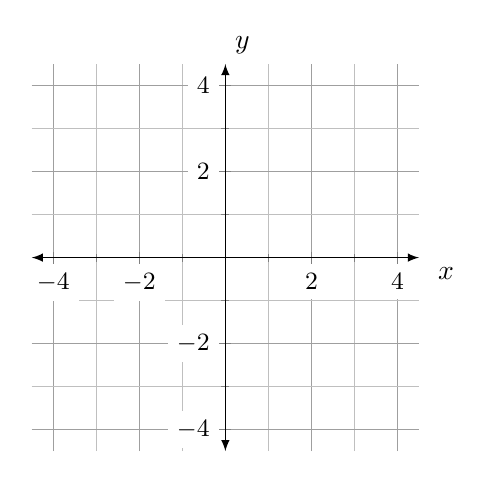
\begin{tikzpicture}[>=latex,scale=1]
				\begin{axis}[
						    width =6.5cm,
					               height=6.5cm,
						    xmin=-4,xmax=4,
						    ymin=-4,ymax=4,
						    grid=both,
						    grid style={line width=.2pt, draw=gray!50},
						    major grid style={line width=.3pt,draw=gray!75},
						    axis lines=middle,
						    minor tick num=1,
						    enlargelimits={abs=0.5},
						    axis line style={latex-latex},
						    ticklabel style={font=\small,fill=white},
						    xlabel={\,\,$x$},
						    ylabel={$y$},
						    xlabel style={below right},
						    ylabel style={above right},
						]
				\end{axis}	
			\end{tikzpicture}
	\end{minipage}
	\begin{minipage}[t]{0.45\linewidth}
		\item[(b)] $\displaystyle g(x)=2\bigg{(}\frac{1}{2}\bigg{)}^2$
		
			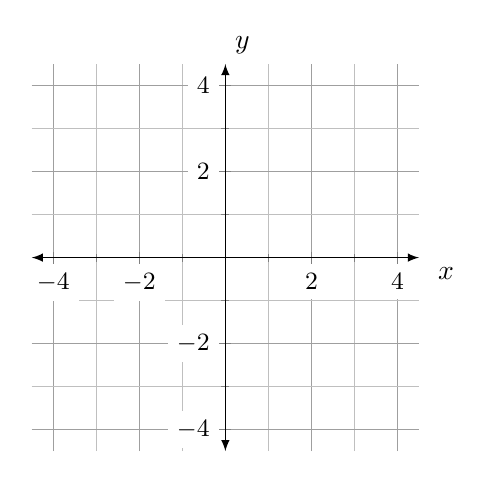
\begin{tikzpicture}[>=latex,scale=1]
				\begin{axis}[
						    width =6.5cm,
					               height=6.5cm,
						    xmin=-4,xmax=4,
						    ymin=-4,ymax=4,
						    grid=both,
						    grid style={line width=.2pt, draw=gray!50},
						    major grid style={line width=.3pt,draw=gray!75},
						    axis lines=middle,
						    minor tick num=1,
						    enlargelimits={abs=0.5},
						    axis line style={latex-latex},
						    ticklabel style={font=\small,fill=white},
						    xlabel={\,\,$x$},
						    ylabel={$y$},
						    xlabel style={below right},
						    ylabel style={above right},
						]
				\end{axis}	
			\end{tikzpicture}
	\end{minipage}
\end{itemize}

\begin{example}
Use a table and graphing calculator to sketch the exponential functions. Tell whether the function shows growth or decay.
\end{example}


\vspace{1cm}


\begin{itemize}
	\begin{minipage}[t]{0.45\linewidth}
		\item[(a)] $f(x)=1.5^x$
		
			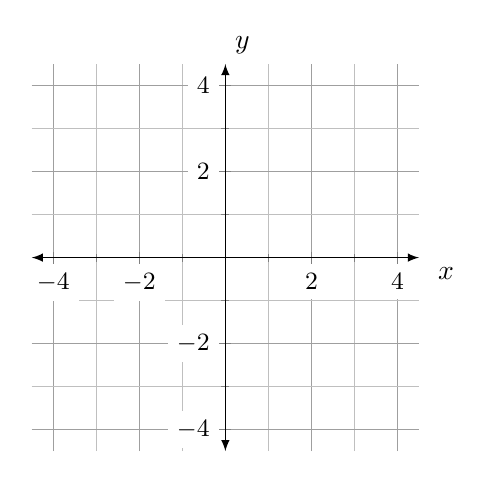
\begin{tikzpicture}[>=latex,scale=1]
				\begin{axis}[
						    width =6.5cm,
					               height=6.5cm,
						    xmin=-4,xmax=4,
						    ymin=-4,ymax=4,
						    grid=both,
						    grid style={line width=.2pt, draw=gray!50},
						    major grid style={line width=.3pt,draw=gray!75},
						    axis lines=middle,
						    minor tick num=1,
						    enlargelimits={abs=0.5},
						    axis line style={latex-latex},
						    ticklabel style={font=\small,fill=white},
						    xlabel={\,\,$x$},
						    ylabel={$y$},
						    xlabel style={below right},
						    ylabel style={above right},
						]
				\end{axis}	
			\end{tikzpicture}
	\end{minipage}
	\begin{minipage}[t]{0.45\linewidth}
		\item[(b)] $g(x)=30(0.8^x)$
		
			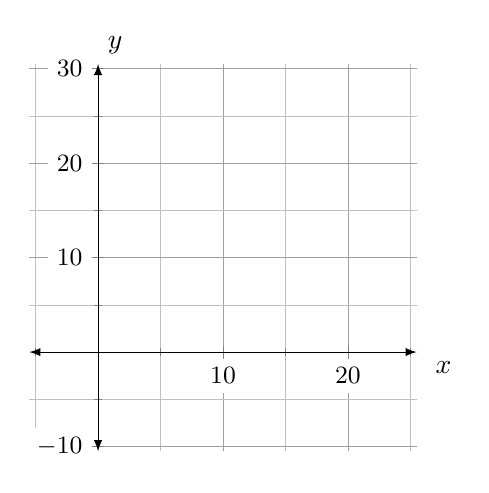
\begin{tikzpicture}[>=latex,scale=1]
				\begin{axis}[
						    width =6.5cm,
					               height=6.5cm,
						    xmin=-5,xmax=25,
						    ymin=-10,ymax=30,
						    grid=both,
						    grid style={line width=.2pt, draw=gray!50},
						    major grid style={line width=.3pt,draw=gray!75},
						    axis lines=middle,
						    minor tick num=1,
						    enlargelimits={abs=0.5},
						    axis line style={latex-latex},
						    ticklabel style={font=\small,fill=white},
						    xlabel={\,\,$x$},
						    ylabel={$y$},
						    xlabel style={below right},
						    ylabel style={above right},
						]
				\end{axis}	
			\end{tikzpicture}
	\end{minipage}
\end{itemize}


\noindent \large \textbf{Exponential Growth Model}

\Large
\[A(x)=P(1 \pm r)^t\]
\normalsize

\noindent Where $A$ is the final amount, $P$ is the principal (initial amount), $r$ is the rate of increase or decrease, and $t$ is time in compounding periods.

\begin{example}
(Calculator) Tyler purchased a rare 1959 Gibson Les Paul guitar in 2000 for $\$12,000$. Experts estimate that its value will increase by $14\%$ per year. Use a calculator to graph to find when the value of the guitar will be $\$60,000$.
\end{example}

\vfill

 \noindent\fbox{\large\textbf{7.1 (day 1) Homework}: page 493 \, 2-5, 7-10 \small } \hfill 
%%%%%%%%%%%%%%%%%%%%%%%%%%%%%%%%%%%%%
%%%%%%%%%%%%%%%%%%%%%%%%%%%%%%%%%%%%%
 \newpage
%%%%%%%%%%%%%%%%%%%%%%%%%%%%%%%%%%%%%
%%%%%%%%%%%%%%%%%%%%%%%%%%%%%%%%%%%%%

\noindent\Large{\textbf{7.1 Exponential Functions (day 2)}}  \\
\indent\hfill\small\noindent \textbf{Objective}: Write and evaluate exponential expressions to model growth and decay situations.\normalsize\\

\noindent Often we have a need to find when two equations are equal or when a function reaches a specific value. This is where we will use the \texttt{INTERSECT} function in the calculate menu.\\

\begin{tabular}[t]{ll}
\indent \underline{Step 1:} & Press \tcbox[size=small, on line]{$Y=$} and use \texttt{Y1} for one side of the equation to solve and \texttt{Y2} for the other \\
&side of the equation.\\
\indent \underline{Step 2:} &  Press \tcbox[size=small, on line]{GRAPH} and use \tcbox[size=small, on line]{WINDOW} to set the \texttt{Xmin} and \texttt{Xmax} as well as the \\
&\texttt{Ymin} and \texttt{Ymax} to fit the interestion within the window.\\
\indent \underline{Step 3:} & Use \tcbox[size=small, on line]{2nd} \tcbox[size=small, on line]{Trace} (the calculate menu) and select option 5. \texttt{insersect}. Press \\
&\tcbox[size=small, on line]{ENTER} on \texttt{Y1} and use the up arrow to select \texttt{Y2}. Use the arrow keys to guess \\
&the approximate intersection of the two curves.\\
\end{tabular}

\vspace{1cm}

\begin{example}
In 1081, the Australian humpback whale population was 350 and has increased at a rate of about $14\%$ each year since then. Write a function to model population growth. Use a graph to predict when the population will reach $20,000$.
\end{example}
\vfill

\begin{example}
The value of a truck bought new for $\$28,000$ decreases $9.5\%$ each year. Write an exponential function, and graph the function. Use the graph to predict when the value will fall to $\$5,000$.
\end{example}
\vfill

\begin{youtry}
A motor scooter purchased for $\$1,000$ depreciates at an annual rate of $15\%$. Write an exponential function, and graph the function. Use the graph to predict when the value will fall below $\$100$.
\end{youtry}
\vfill

%%%%%%%%%%%%%%%%%%%%%%%%%%%%%%%%%%%%%
%%%%%%%%%%%%%%%%%%%%%%%%%%%%%%%%%%%%%
 \newpage
%%%%%%%%%%%%%%%%%%%%%%%%%%%%%%%%%%%%%
%%%%%%%%%%%%%%%%%%%%%%%%%%%%%%%%%%%%%

\begin{example}
The amount of freight transported by rail in the United States was about 580 billion \emph{ton-miles} in 1960 and has been increasing at a rate of $2.32\%$ per year since then.
\end{example}
\begin{itemize}
\item[a.] Write a function representing the amount of freight, in billions of ton-miles, transported annually\\ (let 1960 = year 0).
\vspace{1.5cm}
\item[b.] Graph the function.
\vspace{1.5cm}
\item[c.] In what year would you predict that the number of ton-miles woud have exceeded or would exceed 1 trillion (1000 billion)?
\end{itemize}
\vfill

\begin{youtry}
A quantity of insulin used to regulate sugar in the bloodstream breaks down by about $5\%$ each minute. A body-weight adjusted does is generally 10 units.
\end{youtry}
\begin{itemize}
\item[a.] Write a function representing the amount of the dose that remains after $t$ minutes.
\vspace{1.5cm}
\item[b.] Graph the function.
\vspace{1.5cm}
\item[c.] About how much insulin remains after 10 minutes?
\vspace{1.5cm}
\item[d.] About how long does it take for half the dose to remain?
\end{itemize}
\vfill

 \noindent\fbox{\large\textbf{7.1 (day 2) Homework}: page 494 \, 15, 17, 21, 22, 27 \small } \hfill 

%%%%%%%%%%%%%%%%%%%%%%%%%%%%%%%%%%%%%
%%%%%%%%%%%%%%%%%%%%%%%%%%%%%%%%%%%%%
 \newpage
%%%%%%%%%%%%%%%%%%%%%%%%%%%%%%%%%%%%%
%%%%%%%%%%%%%%%%%%%%%%%%%%%%%%%%%%%%%

%%%%%%%%%%%%%%%%%%%%%%%%%%%%%%%
%%%%%%%%%%%%%%%%%%%%%%%%%%%%%%%
%%%%%%   Section 7.2   %%%%%%%%
%%%%%%%%%%%%%%%%%%%%%%%%%%%%%%%
%%%%%%%%%%%%%%%%%%%%%%%%%%%%%%%
 \section{Inverse of Relations and Functions }
 \indent\hfill\small\noindent \textbf{Objective}: Graph and recognize inverses of relations and functions. Find Inverses of functions\normalsize\\
 \setcounter{example}{0}
 \setcounter{definition}{0}
 %%%%%%%%%%%%%%%%%%%%%%%%%%%%%%%%
 %%%%%%%%%%%%%%%%%%%%%%%%%%%%%%%%

\vspace{-0.5cm}

\begin{definition}
An \textbf{inverse relation} is a relation that swaps $x$ and $y$ in every ordered pair of a given relation. This is the same as reflecting a graph over the line $y=x$.
\end{definition}

\begin{example}
Graph the relation and connect the points. Then graph the inverse relation, identify the domain and range of each relation.
\end{example}
\large

\begin{flushleft}
\underline{Relation}\\
\vspace{0.25cm}

Domain:\\
\vspace{0.25cm}

Range:\\
\vspace{0.5cm}

\rule{3cm}{0.01cm}\\
\underline{Inverse Relation}\\
\vspace{0.25cm}

Domain:\\
\vspace{0.25cm}

Range:\\
\end{flushleft}
\hfill
\vspace{-6cm}
\begin{center}
	\begin{tabular}[t]{|c|c|c|c|c|c|}
	\hline
		&&&&&\\
		$\mathbf{x}$ & 0 & 1 & 2 & 4 &  8 \\
	\hline
		&&&&&\\
		$\mathbf{y}$ & 2 & 4 & 5 & 6 &  7 \\
	\hline
	\end{tabular}
\end{center}
\hfill
\vspace{-3.5cm}
\begin{flushright}
	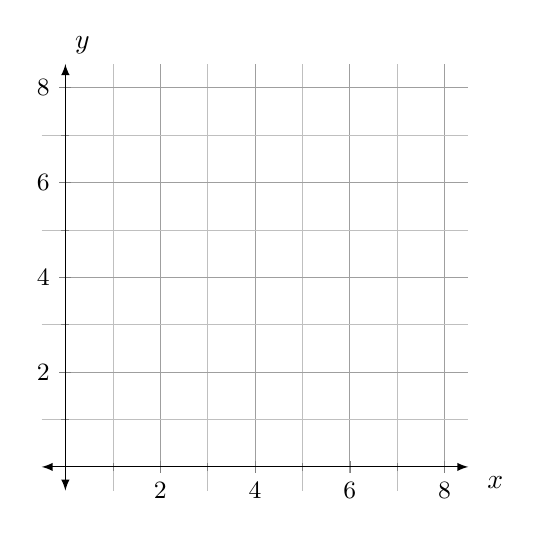
\begin{tikzpicture}[>=latex,scale=1]
		\begin{axis}[
				    width =7cm,
			               height=7cm,
				    xmin=0,xmax=8,
				    ymin=0,ymax=8,
				    grid=both,
				    grid style={line width=.2pt, draw=gray!50},
				    major grid style={line width=.3pt,draw=gray!75},
				    axis lines=middle,
				    minor tick num=1,
				    enlargelimits={abs=0.5},
				    axis line style={latex-latex},
				    ticklabel style={font=\small,fill=white},
				    xlabel={\,\,$x$},
				    ylabel={$y$},
				    xlabel style={below right},
				    ylabel style={above right},
				]
		\end{axis}	
	\end{tikzpicture}
\end{flushright}

\normalsize
\vfill

\begin{youtry}
Graph the relation and connect the points. Then graph the inverse relation, identify the domain and range of each relation.
\end{youtry}
\large

\begin{flushleft}
\underline{Relation}\\
\vspace{0.25cm}

Domain:\\
\vspace{0.25cm}

Range:\\
\vspace{0.5cm}

\rule{3cm}{0.01cm}\\
\underline{Inverse Relation}\\
\vspace{0.25cm}

Domain:\\
\vspace{0.25cm}

Range:\\
\end{flushleft}
\hfill
\vspace{-6cm}
\begin{center}
	\begin{tabular}[t]{|c|c|c|c|c|c|}
	\hline
		&&&&&\\
		$\mathbf{x}$ & 1 & 3 & 4 & 5 & 6 \\
	\hline
		&&&&&\\
		$\mathbf{y}$ & 0 & 1 & 2 & 3 & 5 \\
	\hline
	\end{tabular}
\end{center}
\hfill
\vspace{-3.5cm}
\begin{flushright}
	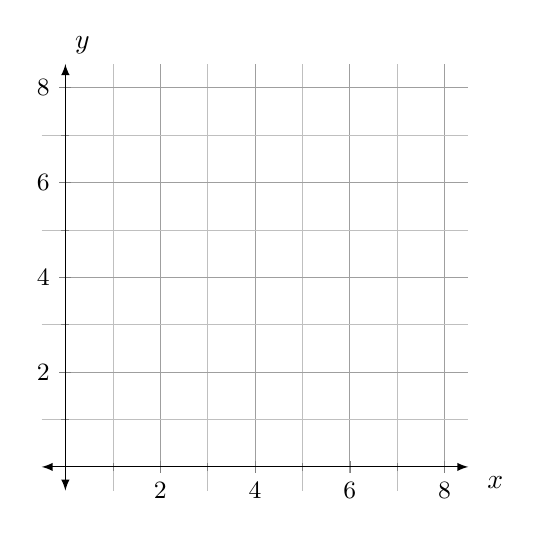
\begin{tikzpicture}[>=latex,scale=1]
		\begin{axis}[
				    width =7cm,
			               height=7cm,
				    xmin=0,xmax=8,
				    ymin=0,ymax=8,
				    grid=both,
				    grid style={line width=.2pt, draw=gray!50},
				    major grid style={line width=.3pt,draw=gray!75},
				    axis lines=middle,
				    minor tick num=1,
				    enlargelimits={abs=0.5},
				    axis line style={latex-latex},
				    ticklabel style={font=\small,fill=white},
				    xlabel={\,\,$x$},
				    ylabel={$y$},
				    xlabel style={below right},
				    ylabel style={above right},
				]
		\end{axis}	
	\end{tikzpicture}
\end{flushright}

\normalsize
\vfill

%%%%%%%%%%%%%%%%%%%%%%%%%%%%%%%%%%%%%
%%%%%%%%%%%%%%%%%%%%%%%%%%%%%%%%%%%%%
 \newpage
%%%%%%%%%%%%%%%%%%%%%%%%%%%%%%%%%%%%%
%%%%%%%%%%%%%%%%%%%%%%%%%%%%%%%%%%%%%


\begin{definition}
When a relation is also a function, you can write the inverse of the function $f(x)$ as $\mathbf{f^{-1}(x)}$. This notation does \underline{not} indicate a reciprocal. Function that undo each other are \textbf{inverse function}.
\end{definition}

\large
\begin{center}
	\begin{tabular}[t]{ccccc}
		\color{blue}\textbf{Input}\color{black}  & $\longrightarrow$ & Function & $\longrightarrow$ & \color{red}\textbf{Output}\color{black} \\
		\color{blue}\textbf{3}\color{black}        & & $\mathbf{f(x)=x+6}$ & & \color{red}\textbf{9}\color{black}\\
		&&&&\\
		\color{red}\textbf{Input}\color{black}  & $\longrightarrow$ & Inverse Function & $\longrightarrow$ & \color{blue}\textbf{Output}\color{black} \\
		\color{red}\textbf{9}\color{black} & & $\mathbf{f^{-1}(x) = x - 6}$ & & \color{blue}\textbf{3}\color{black}\\
	\end{tabular}

\end{center}
\normalsize

%

\begin{example}
Use inverse operations to write the inverse of the following functions.
\end{example}

\begin{minipage}[t]{0.45\linewidth}
(a) $f(x)=\displaystyle\frac{x}{3}$
\end{minipage}
\hfill
\begin{minipage}[t]{0.45\linewidth}
(b) $g(x)=x-\displaystyle\frac{2}{3}$
\end{minipage}
\vfill

%

\begin{youtry}
Use inverse operations to write the inverse of the following functions.
\end{youtry}

\begin{minipage}[t]{0.45\linewidth}
(a) $f(x)=-5x$
\end{minipage}
\hfill
\begin{minipage}[t]{0.45\linewidth}
(b) $g(x)=x+5$
\end{minipage}
\vfill

%

\begin{example}
Write and graph the inverse of each function.
\end{example}

\begin{minipage}[t]{0.45\linewidth}
(a) $f(x)=3x+6$

\vspace{3cm}

	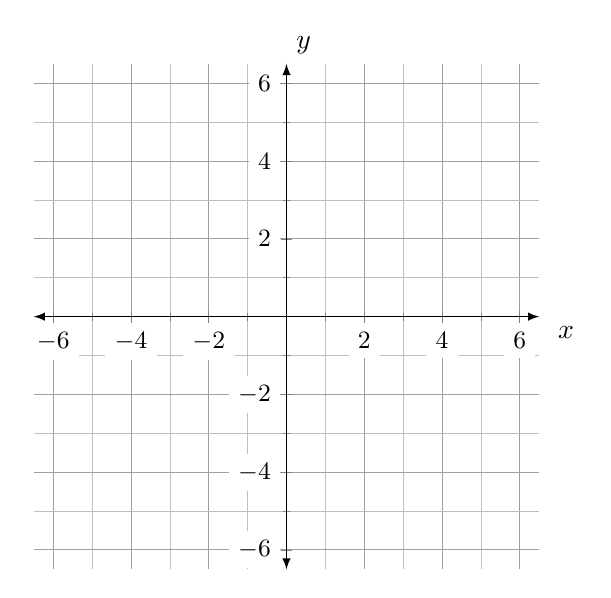
\begin{tikzpicture}[>=latex,scale=1]
		\begin{axis}[
				    width =8cm,
			               height=8cm,
				    xmin=-6,xmax=6,
				    ymin=-6,ymax=6,
				    grid=both,
				    grid style={line width=.2pt, draw=gray!50},
				    major grid style={line width=.3pt,draw=gray!75},
				    axis lines=middle,
				    minor tick num=1,
				    enlargelimits={abs=0.5},
				    axis line style={latex-latex},
				    ticklabel style={font=\small,fill=white},
				    xlabel={\,\,$x$},
				    ylabel={$y$},
				    xlabel style={below right},
				    ylabel style={above right},
				]
		\end{axis}	
	\end{tikzpicture}


\end{minipage}
\hfill
\begin{minipage}[t]{0.45\linewidth}
(b) $g(x)=\displaystyle\frac{2}{3}x+2$

\vspace{3cm}


	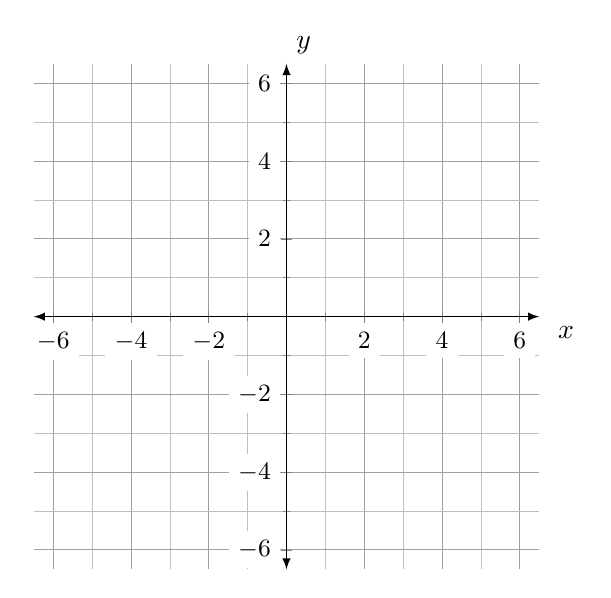
\begin{tikzpicture}[>=latex,scale=1]
		\begin{axis}[
				    width =8cm,
			               height=8cm,
				    xmin=-6,xmax=6,
				    ymin=-6,ymax=6,
				    grid=both,
				    grid style={line width=.2pt, draw=gray!50},
				    major grid style={line width=.3pt,draw=gray!75},
				    axis lines=middle,
				    minor tick num=1,
				    enlargelimits={abs=0.5},
				    axis line style={latex-latex},
				    ticklabel style={font=\small,fill=white},
				    xlabel={\,\,$x$},
				    ylabel={$y$},
				    xlabel style={below right},
				    ylabel style={above right},
				]
		\end{axis}	
	\end{tikzpicture}
\end{minipage}



\vfill
\noindent\fbox{\large\textbf{7.2 Homework (day 1)}: page 501 \, 2-16 all\small }
 
%%%%%%%%%%%%%%%%%%%%%%%%%%%%%%%%%%%%%
%%%%%%%%%%%%%%%%%%%%%%%%%%%%%%%%%%%%%
 \newpage
%%%%%%%%%%%%%%%%%%%%%%%%%%%%%%%%%%%%%
%%%%%%%%%%%%%%%%%%%%%%%%%%%%%%%%%%%%%

%%%%%%%%%%%%%%%%%%%%%%%%%%%%%%%
%%%%%%%%%%%%%%%%%%%%%%%%%%%%%%%
%%%%%%   Section 7.3   %%%%%%%%
%%%%%%%%%%%%%%%%%%%%%%%%%%%%%%%
%%%%%%%%%%%%%%%%%%%%%%%%%%%%%%%
 \section{ Logarithmic Functions  }
  \indent\hfill\small\noindent \textbf{Objective}: Write equivalent forms for exponential and logarithmic functions. \normalsize\\
 \setcounter{example}{0}
 \setcounter{definition}{0}
 %%%%%%%%%%%%%%%%%%%%%%%%%%%%%%%%
 %%%%%%%%%%%%%%%%%%%%%%%%%%%%%%%%
 
\hspace{-0.5cm}\begin{minipage}[t]{0.45\linewidth}
	 \begin{example}

	 \end{example}
	 \begin{itemize}
	 	\item[(a)] 
	 \end{itemize}
\end{minipage}
\hspace{1.25cm}
 \begin{minipage}[t]{0.45\linewidth}
 	 \begin{youtry}

 	 \end{youtry}
	 \begin{itemize}
	 	\item[(b)]
	 \end{itemize}
\end{minipage}
 \vfill
 \begin{example}

 \end{example}
 
\begin{minipage}[t]{0.45\linewidth}
(a) 
\end{minipage}
 \hfill
 \begin{minipage}[t]{0.45\linewidth}
(b) 
\end{minipage}
\vfill
 \vfill
 
 \begin{example}

 \end{example}
\begin{minipage}[t]{0.45\linewidth}
(a) 
\end{minipage}
 \hfill
\begin{minipage}[t]{0.45\linewidth}
(b) 
\end{minipage}
\vfill
\begin{example}

\end{example}

\begin{minipage}[t]{0.45\linewidth}
(a) 
\end{minipage}
 \hfill
\begin{minipage}[t]{0.45\linewidth}
(b) 
\end{minipage}
\vfill

 
 \noindent\fbox{\large\textbf{7.3 (day 1) Homework}: page  \small }
 
 
%%%%%%%%%%%%%%%%%%%%%%%%%%%%%%%%%%%%%
%%%%%%%%%%%%%%%%%%%%%%%%%%%%%%%%%%%%%
 \newpage
%%%%%%%%%%%%%%%%%%%%%%%%%%%%%%%%%%%%%
%%%%%%%%%%%%%%%%%%%%%%%%%%%%%%%%%%%%%

\noindent\Large{\textbf{7.3 (day 2)}} 
  \indent\hfill\small\noindent \textbf{Objective}: Write, evaluate, and graph logarithmic functions.  \normalsize\\

 
 \begin{youtry}

 \end{youtry}
 
\begin{minipage}[t]{0.45\linewidth}
(a) 
\end{minipage}
 \hfill
 \begin{minipage}[t]{0.45\linewidth}
(b) 
\end{minipage}
\vfill
\vfill
 
 \begin{example}

 \end{example}
\begin{minipage}[t]{0.45\linewidth}
(a) 
\end{minipage}
 \hfill
\begin{minipage}[t]{0.45\linewidth}

(b)
\end{minipage}
\vfill

\begin{example}
\end{example}

\begin{minipage}[t]{0.45\linewidth}
(a) 
\end{minipage}
 \hfill
\begin{minipage}[t]{0.45\linewidth}
(b) 
\end{minipage}
\vfill

 
 \noindent\fbox{\large\textbf{7.3 (day 2) Homework}: page  \small }


%%%%%%%%%%%%%%%%%%%%%%%%%%%%%%%%%%%%%
%%%%%%%%%%%%%%%%%%%%%%%%%%%%%%%%%%%%%
 \newpage
%%%%%%%%%%%%%%%%%%%%%%%%%%%%%%%%%%%%%
%%%%%%%%%%%%%%%%%%%%%%%%%%%%%%%%%%%%%
\rhead{Algebra 2: Section  \getcurrentref{chapter}.\getcurrentref{section}}
%%%%%%%%%%%%%%%%%%%%%%%%%%%%%%%
%%%%%%%%%%%%%%%%%%%%%%%%%%%%%%%
%%%%%%   Section 7.4   %%%%%%%%
%%%%%%%%%%%%%%%%%%%%%%%%%%%%%%%
%%%%%%%%%%%%%%%%%%%%%%%%%%%%%%%
 \section{Properties of Logarithms}
 \indent\hfill\small\noindent \textbf{Objective}:  Use properties to simplify logarithmic expressions. \normalsize\\
 \setcounter{example}{0}
 \setcounter{definition}{0}
 %%%%%%%%%%%%%%%%%%%%%%%%%%%%%%%%
 %%%%%%%%%%%%%%%%%%%%%%%%%%%%%%%%
 
\begin{example}
\end{example}
\begin{minipage}[t]{0.45\linewidth}
 (a) 
\end{minipage}
\begin{minipage}[t]{0.45\linewidth}
 (b) 
\end{minipage}
\vfill

\begin{example}

\end{example}
\begin{minipage}[t]{0.45\linewidth}
 (a) 
\end{minipage}
\begin{minipage}[t]{0.45\linewidth}
 (b) 
\end{minipage}
\vfill
\begin{youtry}

\end{youtry}
\begin{minipage}[t]{0.45\linewidth}
 (a) 
\end{minipage}
\begin{minipage}[t]{0.45\linewidth}
 (b) 
\end{minipage}
\vfill

\vfill
 \noindent\fbox{\large\textbf{7.4 (day 1) Homework}: page   \small }
%%%%%%%%%%%%%%%%%%%%%%%%%%%%%%%%%%%%%
%%%%%%%%%%%%%%%%%%%%%%%%%%%%%%%%%%%%%
 \newpage
%%%%%%%%%%%%%%%%%%%%%%%%%%%%%%%%%%%%%
%%%%%%%%%%%%%%%%%%%%%%%%%%%%%%%%%%%%%

\noindent\Large{\textbf{7.4 (day 2) Properties of Logarithms}} 
\indent\hfill\small\noindent \textbf{Objective}: Translate between logarithms in any base.  \normalsize\\

\begin{example}

\end{example}

\begin{minipage}[t]{0.45\linewidth}
 (a) 
\end{minipage}
\begin{minipage}[t]{0.45\linewidth}
 (b) 
\end{minipage}
\vfill

\begin{youtry}

\end{youtry}

\begin{minipage}[t]{0.45\linewidth}
 (a) 
\end{minipage}
\begin{minipage}[t]{0.45\linewidth}
 (b) 
\end{minipage}
\vfill



\vfill
 \noindent\fbox{\large\textbf{7.4 (day 2) Homework}: page   \small }
%%%%%%%%%%%%%%%%%%%%%%%%%%%%%%%%%%%%%
%%%%%%%%%%%%%%%%%%%%%%%%%%%%%%%%%%%%%
 \newpage
%%%%%%%%%%%%%%%%%%%%%%%%%%%%%%%%%%%%%
%%%%%%%%%%%%%%%%%%%%%%%%%%%%%%%%%%%%%

%%%%%%%%%%%%%%%%%%%%%%%%%%%%%%%
%%%%%%%%%%%%%%%%%%%%%%%%%%%%%%%
%%%%%%   Section 7.6   %%%%%%%%
%%%%%%%%%%%%%%%%%%%%%%%%%%%%%%%
%%%%%%%%%%%%%%%%%%%%%%%%%%%%%%%
\setcounter{section}{5}
\rhead{Algebra 2: Section  \getcurrentref{chapter}.\getcurrentref{section}}
 \section{ The Natural Base, $e$}
 \indent\hfill\small\noindent \textbf{Objective}: Use the number $e$ to write and graph exponential functions representing real-world.\normalsize\\
 \setcounter{example}{0}
 \setcounter{definition}{0}
 %%%%%%%%%%%%%%%%%%%%%%%%%%%%%%%%
 %%%%%%%%%%%%%%%%%%%%%%%%%%%%%%%%
 \begin{example}
 \end{example}
 
 \begin{minipage}[t]{0.45\linewidth}
 (a) 
 \end{minipage}
 \hfill
 \begin{minipage}[t]{0.45\linewidth}
 (b) 
 \end{minipage}
\vfill

 \begin{youtry}

 \end{youtry}
 
 \begin{minipage}[t]{0.45\linewidth}
 (a) 
 \end{minipage}
 \hfill
 \begin{minipage}[t]{0.45\linewidth}
 (b) 
 \end{minipage}
\vfill

\begin{definition}
\end{definition}

\begin{example}

\end{example}

\begin{minipage}[t]{0.45\linewidth}
(a) 
\end{minipage}
\hfill
\begin{minipage}[t]{0.45\linewidth}
(b) 
\end{minipage}


\vfill
\noindent\fbox{\large\textbf{7.6 Homework (day 1)}: page  \small }
%%%%%%%%%%%%%%%%%%%%%%%%%%%%%%%%%%%%%
%%%%%%%%%%%%%%%%%%%%%%%%%%%%%%%%%%%%%
 \newpage
%%%%%%%%%%%%%%%%%%%%%%%%%%%%%%%%%%%%%
%%%%%%%%%%%%%%%%%%%%%%%%%%%%%%%%%%%%%

\noindent \Large \textbf{7.6 The Natural Base, $e$ (day 2)} \normalsize
 \indent\hfill\small\noindent \textbf{Objective}: Solve equations and problems involving $e$ or natural logarithms.\normalsize\\

\begin{example}

\end{example}
\vfill

\begin{example}

\end{example}
(a) 
\vfill

(b) 


\vfill
\noindent\fbox{\large\textbf{7.6 Homework (day 2)}: page \small }
%%%%%%%%%%%%%%%%%%%%%%%%%%%%%%%%%%%%%
%%%%%%%%%%%%%%%%%%%%%%%%%%%%%%%%%%%%%
 \newpage
%%%%%%%%%%%%%%%%%%%%%%%%%%%%%%%%%%%%%
%%%%%%%%%%%%%%%%%%%%%%%%%%%%%%%%%%%%%

%%%%%%%%%%%%%%%%%%%%%%%%%%%%%%%
%%%%%%%%%%%%%%%%%%%%%%%%%%%%%%%
%%%%%%   Section 7.7   %%%%%%%%
%%%%%%%%%%%%%%%%%%%%%%%%%%%%%%%
%%%%%%%%%%%%%%%%%%%%%%%%%%%%%%%
 \section{Transforming Exponential and Logarithmic Functions }
 \noindent \hfill\small \noindent \textbf{Objective}: Transform exponential and logarithmic functions by changing parameters.. \normalsize\\
 \setcounter{example}{0}
 \setcounter{definition}{0}
 %%%%%%%%%%%%%%%%%%%%%%%%%%%%%%%%
 %%%%%%%%%%%%%%%%%%%%%%%%%%%%%%%%

\begin{example}

\end{example}

\begin{minipage}[t]{0.45\linewidth}
(a)  
\end{minipage}
\hfill
\begin{minipage}[t]{0.45\linewidth}
(b) 
\end{minipage}

\vfill

\begin{example}

\end{example}

\begin{minipage}[t]{0.45\linewidth}
(a) 
\end{minipage}
\hfill
\begin{minipage}[t]{0.45\linewidth}
(b) 
\end{minipage}


\vfill
\vfill
 \noindent\fbox{\large\textbf{7.7 Homework (day 1)}: page  \small }
%%%%%%%%%%%%%%%%%%%%%%%%%%%%%%%%%%%%%
%%%%%%%%%%%%%%%%%%%%%%%%%%%%%%%%%%%%%
 \newpage
%%%%%%%%%%%%%%%%%%%%%%%%%%%%%%%%%%%%%
%%%%%%%%%%%%%%%%%%%%%%%%%%%%%%%%%%%%%

\noindent\Large\textbf{7.7 Transforming Exponential and Logarithmic Functions (day 2)}\\
\noindent \hfill\small \noindent \textbf{Objective}: Describe the effects of changes in the coefficients of exponential and logarithmic functions. \normalsize\\

\begin{example}
\end{example}

\begin{minipage}[t]{0.45\linewidth}
(a)  
\end{minipage}
\hfill
\begin{minipage}[t]{0.45\linewidth}
(b) 
\end{minipage}

\vfill

\begin{example}

\end{example}
\vfill


\begin{example}

\end{example}


\vfill
\noindent\fbox{\large\textbf{7.7 Homework (day 2)}: page }
%%%%%%%%%%%%%%%%%%%%%%%%%%%%%%%%%%%%%
%%%%%%%%%%%%%%%%%%%%%%%%%%%%%%%%%%%%%
 \newpage
%%%%%%%%%%%%%%%%%%%%%%%%%%%%%%%%%%%%%
%%%%%%%%%%%%%%%%%%%%%%%%%%%%%%%%%%%%%


%%%%%%%%%%%%%%%%%%%%%%%%%%%%%%%
%%%%%%%%%%%%%%%%%%%%%%%%%%%%%%%
%%%%%%   Chapter 7 Review   %%%%%%%%
%%%%%%%%%%%%%%%%%%%%%%%%%%%%%%%
%%%%%%%%%%%%%%%%%%%%%%%%%%%%%%%
\rhead{Algebra 2: Chapter \getcurrentref{chapter} Review} 
\hspace{-1.6cm} \noindent\Large\textbf{Chapter 7 Review (day 1)}\large
 %%%%%%%%%%%%%%%%%%%%%%%%%%%%%%%%
 %%%%%%%%%%%%%%%%%%%%%%%%%%%%%%%%

\begin{enumerate}


	\begin{minipage}[t]{0.45\linewidth}
		\item .
	\end{minipage}
	\hfill
	\begin{minipage}[t]{0.45\linewidth}
		\item .
	\end{minipage}
	\vspace{3cm}
	
\hspace{-2cm}  \\

	\begin{minipage}[t]{0.45\linewidth}
		\item  .
	\end{minipage}
	\hfill
	\begin{minipage}[t]{0.45\linewidth}
		\item .
	\end{minipage}
	\vspace{3cm}
	
\hspace{-2cm}  \\

	\begin{minipage}[t]{0.45\linewidth}
		\item .
	\end{minipage}
	\hfill
	\begin{minipage}[t]{0.45\linewidth}
		\item .
	\end{minipage}
	
	\vspace{4cm}
	
	\begin{minipage}[t]{0.45\linewidth}
		\item .
	\end{minipage}
	\hfill
	\begin{minipage}[t]{0.45\linewidth}
		\item .
	\end{minipage}
	
	\vspace{4cm}
	
	\begin{minipage}[t]{0.45\linewidth}
		\item .
	\end{minipage}
	\hfill
	\begin{minipage}[t]{0.45\linewidth}
		\item .
	\end{minipage}




\vfill

%%%%%%%%%%%%%%%%%%%%%%%%%%%%%%%%%%%%%
%%%%%%%%%%%%%%%%%%%%%%%%%%%%%%%%%%%%%
 \newpage
%%%%%%%%%%%%%%%%%%%%%%%%%%%%%%%%%%%%%
%%%%%%%%%%%%%%%%%%%%%%%%%%%%%%%%%%%%%

\hspace{-2cm} 

	\begin{minipage}[t]{0.45\linewidth}
		\item .
	\end{minipage}
	\hfill
	\begin{minipage}[t]{0.45\linewidth}
		\item .
	\end{minipage}
	
	\vspace{4cm}
	
	\begin{minipage}[t]{0.45\linewidth}
		\item .
	\end{minipage}
	\hfill
	\begin{minipage}[t]{0.45\linewidth}
		\item .
	\end{minipage}
	
		\vspace{4cm}
	
\hspace{-2cm} 
	
	\begin{minipage}[t]{0.45\linewidth}
		\item .
	\end{minipage}
	\hfill
	\begin{minipage}[t]{0.45\linewidth}
		\item .
	\end{minipage}
	
	\vspace{4cm}


%%%%%%%%%%%%%%%%%%%%%%%%%%%%%%%%%%%%%
%%%%%%%%%%%%%%%%%%%%%%%%%%%%%%%%%%%%%
 \newpage
%%%%%%%%%%%%%%%%%%%%%%%%%%%%%%%%%%%%%
%%%%%%%%%%%%%%%%%%%%%%%%%%%%%%%%%%%%%


\hspace{-2cm}\noindent \hfill \textbf{Ch 7 Review (day 2)}\\ \normalsize



\end{enumerate}

\end{document}










